\chapter{Introducción}

El 12 de octubre de 1492 un temerario explorador, Cristobal Colón, y su tripulación pisan la arena de una isla muy al oeste de Europa conocida como Guanahani. Este hecho marca un hito en la historia de la humanidad pues los cambios culturales, económicos, políticos y militares que produce dan lugar a la llamada Edad Moderna.

Colón vio una oportunidad de negocio en el control de las rutas comerciales que unían Europa con Asia pues eran recorridas por miles de comerciantes que traían especias y productos de lujo desde las tierras de Extremo Oriente. El comercio además se realizaba por tierra, lo que lo convertía en un proceso lento, inseguro e ineficiente, además de enriquecedor para los árabes que controlaban las rutas comerciales.

El proyecto tenía un gran interés económico pues como se ha dicho anteriormente, el control de una ruta comercial con Asia era muy lucrativo, pero a su vez tenía un gran riesgo ya que el futuro de la expedición era tremendamente incierto y había pocas posibilidades de encomendarse al vasto océano y volver para contarlo. Debido a esta incertidumbre sobre el retorno de la inversión a Colón le fue complicado encontrar financiación para su proyecto, hasta que finalmente, tras recurrir a varios monarcas y mecenas,  los Reyes Católicos le proveyeron de los recursos necesarios para iniciar su aventura.

Se podría considerar a Cristobal Colón como un emprendedor, a pesar de que el término fue usado por primera vez doscientos años después por el economista Richard Cantillon que define al emprendedor como 

\begin{itquote}
	La persona que paga un cierto precio para revender un producto a un precio incierto, por ende tomando decisiones acerca de la obtención y el uso de recursos, y admitiendo consecuentemente el riesgo en el emprendimiento.
 	\begin{flushright}
 	\cite[pág 21]{ashokbhanudasnavale2013}.
 	\end{flushright}
\end{itquote}

De esta definición se puede apreciar que un emprendedor inicia proyectos y acepta la incertidumbre y el riesgo que ello conlleva, puesto que en caso de desastre es él quien asume la responsabilidad.

La actitud emprendedora ha sido una constante a lo largo de la historia de la humanidad: desde Cristobal Colón hasta Bill Gates, pasando por Leonardo Da Vinci, Henry Ford o Nikola Tesla; hombres y mujeres con coraje han empezado proyectos bajo una idea prometedora y asumiendo grandes riesgos, motivados por la pasión y las perspectivas de éxito. 

El emprendimiento es una actividad especialmente necesaria para el progreso de una sociedad pues es un proceso que crea riqueza, innovación y empleo. Los emprendedores crean productos y servicios revolucionarios que hacen la vida de las personas más fácil, mejorando por ello su calidad de vida. Además suele ser una opción frecuente en épocas de crisis económicas debido a la escasez de empleo.

\section{Emprendimiento y el fenómeno startup}

Cada vez es más frecuente escuchar el término \textquote{startup}, pequeñas empresas dedicadas al ámbito tecnológico que alcanzan en pocos años grandes cuotas de mercado y se venden por cantidades astronómicas a empresas más grandes.

El fenómeno goza de tanta popularidad que ha inspirado incluso a series televisivas como \textquote{Silicon Valley}\footnote{\url{http://www.imdb.com/title/tt2575988/?ref_=nv_sr_1}}, que narra las aventuras de un grupo de jóvenes ingenieros que crean una \textquote{startup} tecnológica y se enfrentan al reto de sobrevivir en un ecosistema hostil como es el mercado; la película \textquote{Piratas de Silicon Valley}, que narra la historia de enfrentamiento entre Microsoft y Apple; la película \textquote{La red social} que cuenta la historia de Mark Zuckerberg y como crea la red social \textquote{Facebook}.

Llegado a este punto cabe preguntarse: ¿Qué es exactamente una \textquote{startup}?. Es un error común pensar que las \textquote{startup} son simplemente versiones más pequeñas de empresas grandes. En palabras de los gurús del emprendimiento Steve Blank y Bob Dorf, \textquote{Una \textquote{startup} es una organización temporal en busca de un modelo de negocio rentable, que pueda repetirse y que es escalable}\cite{steveblankbobdorf2013}.

De la anterior definición se puede extraer que una \textquote{startup}:
\begin{itemize}
	\item Es una organización temporal, es decir, el objetivo no es ser siempre una \textquote{startup}. El objetivo es convertirse en una empresa consolidada.
	\item No conoce con seguridad cual va a ser su actividad. En su lugar parten de un modelo de negocio temporal que va evolucionando a medida que interactúa con el mercado.
	\item Busca un modelo de negocio repetible y escalable, que le permita ejecutar dicho modelo de negocio durante un tiempo indefinido y además expandirse.
\end{itemize}
El emprendimiento es inherente al fenómeno \textquote{startup} pues la incertidumbre es un pilar fundamental al crear una de estas empresas, que ni siquiera tienen un modelo de negocio que se pueda asegurar que va a funcionar.

\section{Estado actual del emprendimiento en España}

Si bien el fenómeno \textquote{startup} nació en EEUU y es allí donde está más consolidado, en España es una tendencia igualmente extendida. Atendiendo a cifras de financiación \textquote{en 2015, las startups españolas lograron financiación por valor de 500 millones de euros, un 87\%   más que en 2014, cuando apenas se invirtieron 286 millones de euros} \cite{albertoiglesiasfraga2016}.

Actualmente en nuestro país hay 1783 empresas emergentes distribuidas principalmente en Madrid, Cataluña y la Comunidad valenciana. Dichas empresas se dedican principalmente al ecommerce(22\%), social media(13\%) y las empresas(12\%). En cuanto a la financiación, 172 inversores operan en el ámbito \textquote{startup} a lo largo de la península \cite{startupxplore2017} y los fondos que han aportado crecen año a año: 

\begin{itquote}
En 2013, tres \textquote{startup} lograron rondas de financiación que superaran los 10 millones de euros [...] en 2014, esta cifra aumentó a cuatro [...] el pasado año la explosión no tuvo parangón, ya que hasta 13 startups lograron capitalizar más de 10 millones de euros para fomentar su desarrollo.
\begin{flushright}\cite{albertoiglesiasfraga2016}. \end{flushright}
%NOTA, si puedes, pon en la cita la página donde lo dice. si no, el capítulo o sección si es electrónico. Si no, pues nada.
\end{itquote}

\section{Lean startup}

\textquote{Lean STARTUP} es un modelo de gestión empresarial dinámico ampliamente utilizado en la creación de empresas emergentes. En contraposición a las metodologías tradicionales,  \textquote{Lean STARTUP} se basa en ciclos de desarrollo cortos que permiten sacar el producto al mercado de forma temprana. De este modo se puede obtener retroalimentación de los clientes en las etapas iniciales de la empresa, lo que da lugar a que el producto cambia y se adapta a las necesidades de los clientes.

El primer paso para crear una \textquote{startup} según esta metodología es plasmar las hipótesis sobre el modelo de negocio en el Lean Canvas (ver fig. \ref{leanCanvas})

\begin{figure}[H]
\begin{center}
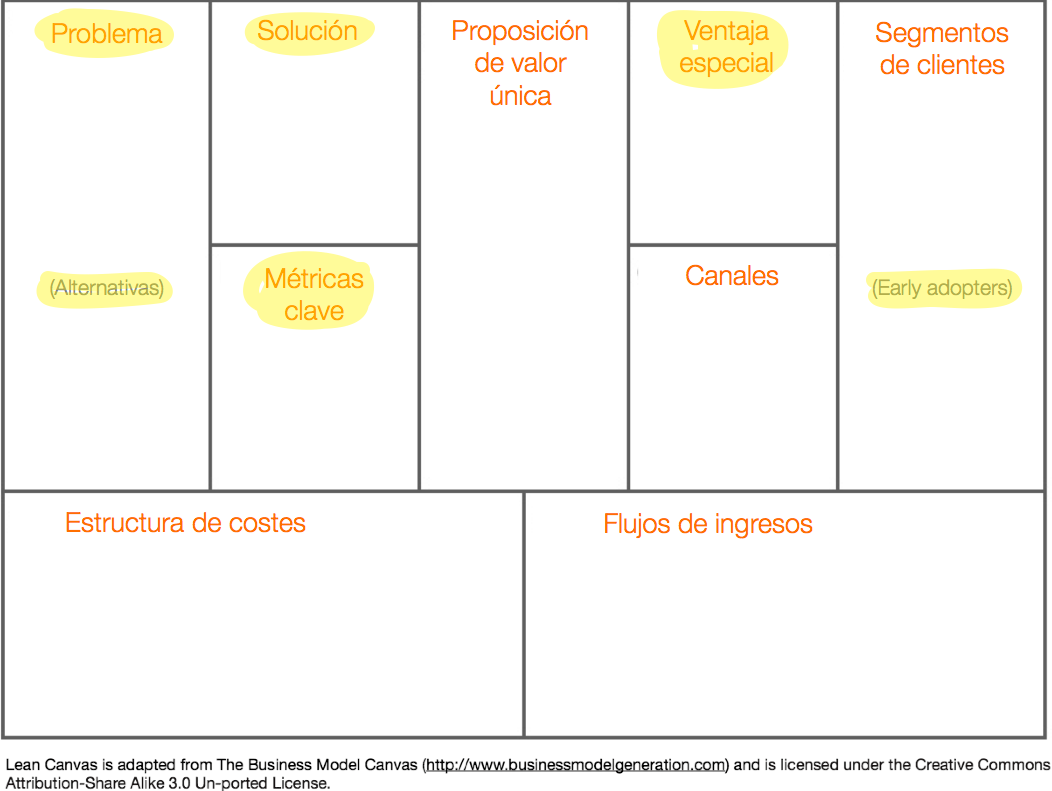
\includegraphics[scale=0.25]{imagenes/lienzo_lean_canvas.png}
\caption{Lienzo propuesto por Ash Maurya para el proceso LEAN STARTUP. Fuente: Blog de Javier Megias. \url{http://javiermegias.com/blog/2012/10/lean-canvas-lienzo-de-modelos-de-negocio-para-startups-emprendedores/} }
\label{leanCanvas}
\end{center}
\end{figure}

Estas hipótesis no conforman el modelo de negocio definivo, si no que irán evolucionando a lo largo de la vida de la empresa de acuerdo al feedback de los clientes. Esta evolución del producto en relación a los deseos del clientes se denomina \textbf{customer development} y es uno de los conceptos claves en Lean startup.

El ciclo de vida de una \textquote{startup} se basa en tres pasos fundamentales que se repiten cíclicamente:
\begin{itemize}
	\item Construir: se diseña el producto en función de las hipótesis que se establecen en el \textbf{lean canvas}. En la primera iteración se crea una versión del producto que tenga las minímas funcionalidades necesarias para aportar valor a los potenciales clientes. Esta versión del producto se denomina \textbf{producto minímo viable}. El objetivo de esta etapa es ''comenzar a recopilar datos y medir resultados. Este modelo de producto no busca ser el resultado final sino un producto suficiente para testar la reacción del potencial cliente" \cite{antevenio2016}.
	\item Medir: tras contrastar nuestras hipótesis de negocio con los clientes a través del \textbf{producto minímo viable} obtenemos información sobre nuestro producto y sobre la propia empresa mediante \textbf{métricas clave}. Dichas métricas (tales como ¿Cuánto cuesta captar un cliente? o ¿Cuánto dinero gastamos mensualmente?) son valoraciones objetivas sobre el rendimiento del producto y de la empresa, y calcularlas de forma periódica es importante ya que permite trazar una evolución y detectar errores y mejoras en la estrategia empresarial.
	\item Aprender: es una etapa clave ya que si el conocimiento obtenido se aplica, se estará más cerca de crear un producto que los clientes quieran comprar. ''este conocimiento adquirido se debe aplicar a un nuevo proceso que comienza de nuevo. Se vuelve a crear un producto, que será una mejora del mismo lo que hace arrancar de nuevo el círculo de crear, medir y aprender" \cite{antevenio2016}. Al llegar a este punto las startups se deben plantear si realizar un pequeño ajuste al producto y volver a \textbf{iterar} o si bien, en caso de que los resultados del producto hayan sido un desastre, hacer cambios de base al modelo de negocio. Estos cambios que afectan a una o más hipótesis del \textbf{lean canvas} se denominan \textbf{pivotar} y consisten en ''cambiar una hipótesis fundamental sobre el producto, la estrategia, y el motor de crecimiento" \cite{emooc}.
\end{itemize}

El proceso se puede realizar cuantas veces sea necesario hasta conseguir el producto que se considere más acorde al cliente. La metodología Lean \textquote{startup} no trata de evitar que fallemos en el primer intento de lanzar al mercado nuestro servicio, sino que trata de que ese fallo nos salga más ‘barato’ al haber empleado una cantidad considerablemente menor de tiempo y de recursos materiales y económicos. \cite{andreapelaez} .

\section{Educación sobre emprendimiento}

Dado que la creación de iniciativas empresariales en un fenómeno cada vez más extendido, ha surgido la necesidad de formar a profesionales que sean capaces de poner en marcha tales proyectos y dirigirlos de forma exitosa. Actualmente existe un gran abanico de opciones formativas, entre las cuales destacaremos los videojuegos. El videojuego, visto como elemento narrativo, supone una poderosa herramienta de comunicación y de experimentación de vivencias. 

El tema alrededor del cual gira este Trabajo fin de grado es el videojuego como elemento de aprendizaje sobre emprendimiento. La creación de un videojuego formativo provee a los futuros alumnos no solo de una formación teórica, si no que permite vivir una experiencia inmersiva en una historia que transmita conocimientos importantes a lo largo de la misma. Además es notablemente más divertido aprender jugando a un videojuego que atendiendo a interminables sesiones teóricas. Incluso se puede considerar como formación práctica el jugar ya que el jugador deberá de poner en acción los conocimientos teóricos previamente aprendidos.




